\documentclass[11pt]{article}
\usepackage{polski}
\usepackage[utf8]{inputenc}
\usepackage[OT4]{fontenc}
\usepackage[pdftex]{graphicx}
\usepackage{amsmath}

\begin{document}
\title{Algorytmy ewolucyjne. Zadanie 2}
\author{Michał Dettlaff, Dariusz Kuziemski}
\maketitle

\section{Wprowadzenie}

\noindent
Celem rozpatrywanego problemu jest porównanie skuteczności 
strategii ewolucyjnej i algorytmu genetycznego w wybranych 
problemach optymalizacji numerycznej.

Funkcjami, z których skorzystamy w eksperymencie - funkcje
ciągłe, potencjalnie trudne do optymalizacji - będą uogólniona 
Funkcja Rosenbrocka oraz uogólniona Funckja Griewanka.

Dotychczas problemami optymalizacji za pomocą strategii
ewolucyjnych zajmowali się m.in. Pedro A. F. Cruz oraz
 Delfim F. M. Torres w swojej pracy 
\textit{Evolution strategies in optimization problems}. 


\section{Metodologia}
\noindent
By porównać skuteczność strategii ewolucyjnej i algorytmu 
genetycznego wykorzystamy \textbf{ Cumulative Step Size Adaptation (CSA)}
(Kumulowana długość kroku) jako przykład strategii oraz 
\textbf{Differential Evolution} (Ewolucja przyrostowa) jako algorytm genetyczny.

Strategie ewolucyjne zostały pomyślane jako narzędzie optymalizacji
parametrycznej. Rozwiązania mają tu postać m-wymiarowych wektorów
o współrzędnych rzeczywistych. Charakterystyczną cechą tej
metaheurystyki jest samoadaptacja parametrów sterujących,
które podlegają ewolucji wraz z właściwymi rozwiązaniami. 
Osiąga się to przez rozszerzenie reprezentacji osobnika,
dołączając do wektora rozwiązania wektor parametrów sterujących.

Algorytmy genetyczne są rodzajem algorytmów przeszukujących
przestrzeń alternatywnych rozwiązań problemu w celu wyszukania 
rozwiązań najlepszych. Ich charakterystyczną cechą jest 
binarne kodowanie rozwiązania jako pojedynczego chromosomu. 
Selekcja wstępna jest realizowana za pomocą mechanizmu selekcji 
proporcjonalnej (algorytm wymaga więc niekiedy odpowiedniego 
przekształcenia funkcji oceny). Wytwarzanie osobników potomnych
jest realizowane przy użyciu krzyżowania prostego oraz 
następującej po nim mutacji równoległej, przy czym krzyżowanie 
jest uważane za mechanizm podstawowy. W algorytmie stosuje się 
pełną wymianę pokoleń, tak więc w każdym cyklu wytwarza się tylu 
osobników potomnych, ile wynosi wielkość populacji. Wyróżnia się 
trzy zasadnicze grupy zastosowań AG: algorytmy przeszukujące 
(Search), optymalizujące (Optimization) i uczące (Learning) 
Wymienione grupy nie są jednak rozłączne i granica między 
nimi jest płynna.

Pierwsza wykorzystana funkcja testowa - funkcja Rosenbrock'a - 
jest funkcją niewypukłą używaną w optymalizacji jako test 
dla algorytmów optymalizacji. Zwana jest też ze względu 
na swój kształt "Doliną Rosenbrocka" lub "Funkcją Banana 
Rosenbrocka". Funkcja ta jest popularnie używana do 
przedstawiania zachowań algorytmów optymalizacji.

\begin{center}
$f(x) = \sum_{i=1}^{n-1} [ 100 ( {x_{i+1} - {x_i}^2} )^2 + (x_i -1)^2]$

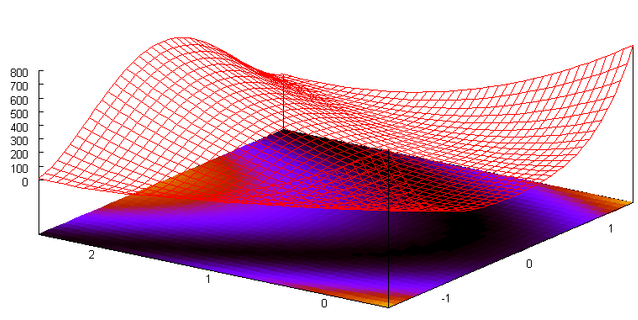
\includegraphics[scale=0.50]{wykres_rosenbrock}\newpage
\end{center}

Drugą funkcją jest Funkcja Griewanka, która funkcją trudną do optymalizacji
z powodu silnej zależności wewnętrznej pomiędzy zmiennymi.
Uogólnioną, n–wymiarową funkcję Griewanka definiuje się następującym wzorem:

\begin{center}
$f(x) = \frac{1}{4000} \sum_{i=1}^n {x_i}^{2} - \prod_{i=1}^n cos(x_i / \sqrt{i}) +1$
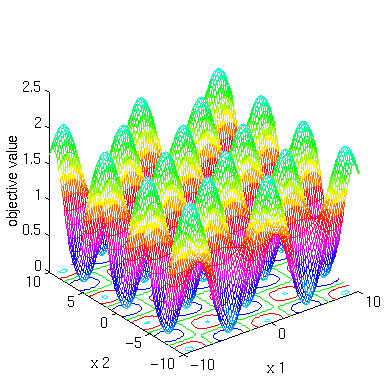
\includegraphics[scale=0.50]{wykres_griewank}\newline
\end{center}

\section{Wyniki}

Funkcja Rosenbrocka\newline
\includegraphics[scale=0.50]{rosenbrock_csa}\newline
\includegraphics[scale=0.50]{rosenbrock_de}\newline

Dla funkcji Rosenbrocka strategia ewolucyjna 
(tj. Kumulowana długość kroku) okazuje się 
skuteczniejsza od algorytmu genetycznego
(tj. Ewolucji przyrostowej) - tzn. szybciej 
znajduje rozwiązanie zadanego problemu optymalizacji. 
Warto jednak zauważyć, że współczynnik zmiany średniego
najlepszego osobnika w populacji zmienia się nierównomiernie
- najbardziej widoczne efekty uzyskujemy dla pierwszych 
pokoleń. Natomiast współczynnik dla algorytmu genetycznego
równomiernie dąży do rozwiązania. 
\newpage

Funkcja Griewanka\newline
\includegraphics[scale=0.50]{griewank_csa}\newline
\includegraphics[scale=0.50]{griewank_de}\newline
\newpage

W przypadku funkcji Griewanka szybsze rozwiązanie
zagadnienia otrzymujemy z wykorzystaniem algorytmu 
genetycznego. Jednak zauważamy idee pododne jak dla
funkcji Rosenbrocka - zastosowana strategia ewolucyjna
zwraca lepsze wyniki dla pokoleń początkowych, podczas
gdy algorytm genetyczny pracuje jednostajnie.

Otrzymane wyniki porównań dla testowanych funckji 
skłaniają do następującego wniosku:
najbardziej efektywne rozwiązania zadań optymalizacji
możemy uzyskać stosująć dla pierwszych pokoleń strategię
ewolucyjną, a następnie algorytm genetyczny.
\newpage

\section{Bibliografia}
Kwaśnicka H.: \textit{Obliczenia ewolucyjne w sztucznej inteligencji.} 
\newline Oficyna Wydawnicza Politechniki Wrocławskiej,Wrocław, 1999. \newline
http://prawo.uni.wroc.pl/\~{}kwasnicki/todownload/prognozowanie\_popytu.pdf \newline
http://www.kirj.ee/public/Phys\_Math/2007/issue\_4/phys-2007-4-3.pdf \newline
http://stefanbrock.neostrada.pl/materialy/NMS/CI\_wyklad\_ewoluc\_2.pdf \newline
http://www.mimuw.edu.pl/\~{}grygiel/archive/dokumenty/notatki.pdf \newline
http://pl.wikipedia.org/wiki/Funkcja\_Rosenbrock'a

\end{document}
